\documentclass[border=2pt]{standalone}
\usepackage{pgfplots}
\pgfplotsset{compat=1.18}
\begin{document}
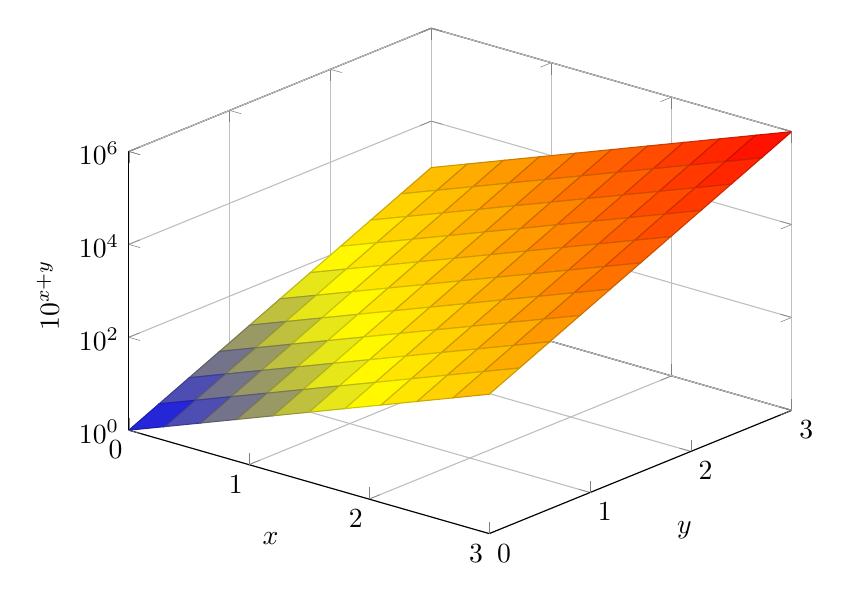
\begin{tikzpicture}
  \begin{axis}[
    width=10cm,
    height=8cm,
    view={40}{30},
    domain=0:3,
    y domain=0:3,
    samples=11,
    zmode=log,
    zmin=1,
    zmax=1000000,
    grid=both,
    xlabel={$x$},
    ylabel={$y$},
    zlabel={$10^{x+y}$}
  ]
    \addplot3[surf] {10^(x+y)};
  \end{axis}
\end{tikzpicture}
\end{document}
